\subsection{Radial velocity method for exoplanet detection}
The radial velocity method is one of the few current methods of detecting exoplanets. Two celestial bodies in orbit around each other, such as a star and a planet, orbit their common center of mass (barycenter). This means that the star, although typically much more massive than the planet, is also in movement relative to an outside observer. The larger the planet is relative to the star, the faster the star will appear to be moving. This motion we can measure through the Doppler effect, as the light of the star observed on Earth will be blue-shifted when the star is moving toward us and red-shifted when moving away. If there is a planet around a star, we should therefor observe a periodic Doppler shift. The method is illustrated in figure \ref{fig:rv_method_illustration}.

\begin{SCfigure}[1][!ht]%
    \begin{wide}  
        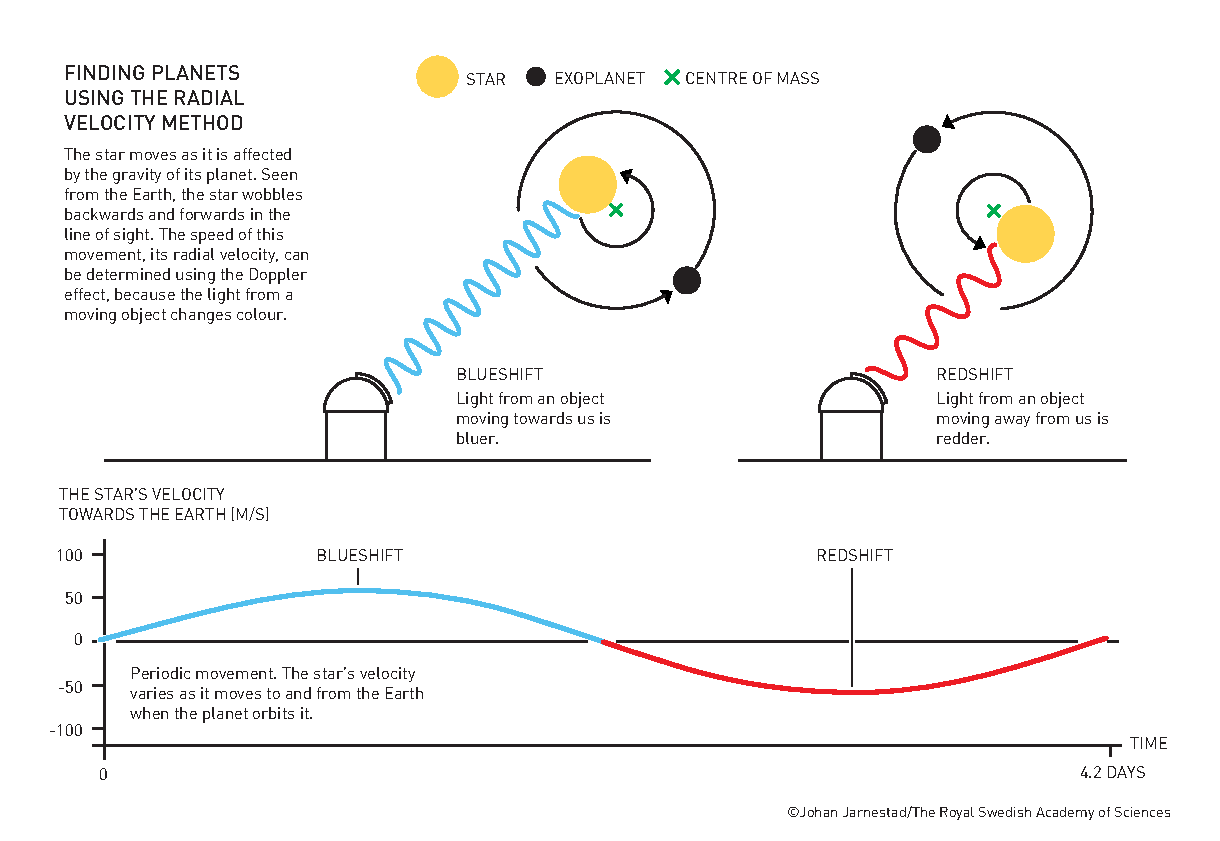
\includegraphics[width=\textwidth]{figures/rv_method_illustration.pdf}
        \caption{Illustration of the radial velocity method for exoplanet detection. © Johan Jarnestad/The Royal Swedish Academy of Sciences.}
        \label{fig:rv_method_illustration}
    \end{wide}
\end{SCfigure}

\vspace{0.5cm}

The induced motion is called \emph{radial velocity semi-amplitude} and can be calculated by 

\begin{equation}
    K_{1}=\sqrt{\frac{G}{\left(1-e^{2}\right)}} m_{2} \sin i\left(m_{1}+m_{2}\right)^{-1 / 2} a^{-1 / 2}
    \label{eq:rv_K}
\end{equation}

where $G$ is Newton's gravitational constant, $e$ is the eccentricity of the orbit, $a$ the semi-major axis, $i$ the inclination and $m_1$ and  $m_2$ the mass of the star and the planet respectively \cite{radial_velocity_techniques}. With this formula, we can calculate that Jupiter causes the Sun to move back and forth with a velocity of $K_1 = 12.5$ m/s, for an outside observer in the plane of orbit, while the Earth induces a radial velocity of only $K_1 = 8.95$ cm/s. If we look at another star system exactly in the plane of orbit the inclination $i$ is 90° degrees. If we however observe the system at an angle (which most of the time we are) the radial velocity will appear smaller by a factor of $\sin{i}$.

\subsubsection{Doppler shift}
The radial velocity method relies on the well-known Doppler effect. Ignoring terms of $c^{-4}$ and higher, the general shift caused by a relative displacement between the source and an observer at zero gravitational potential is given by 

\begin{equation}
    \label{eq:doppler_GR_SR}
    \lambda=\lambda_{0} \frac{1+\frac{1}{c} \mathbf{k} \cdot \mathbf{v}}{1-\frac{\Phi}{c^{2}}-\frac{v^{2}}{2 c^{2}}},
\end{equation}

where $\lambda$ is the observed wavelength, $\lambda_0$ the emitted wavelength, $\Phi$ the Newtonian gravitational potential at the source $(\Phi=G M / r$ at a distance $r$ of a spherically symmetric mass $M$ ), $\textbf{k}$ the unit vector pointing from the observer to the source, $\textbf{v}$ the velocity of the source relative to the observer and $c$ the speed of light. This formula accounts for both special relativistic effects and the gravitational Doppler shift described by general relativity\cite{doppler_shift_GR_formula}.
 
As we are dealing with velocity shifts on the order of meters or centimeters per second, we can safely ignore special relativistic effects and thus cross out the third term in the denominator. The gravitational Doppler shift is independent of the motion of the star but instead depends on its mass and radius. The Sun has a mass loss rate of about $3 \times 10^{-12}$ \% per year\cite{carroll2017introduction}. If we assume a similar mass loss rate for the stars used in this study (which all have masses close to that of the Sun), we can safely assume that the gravitational effect is constant, and since we are computing only relative shifts we can ignore it and omit the second term from the denominator.

If the unit vector $\textbf{k}$ were pointing directly toward us, it would mean that we were observing the system in the plane of orbit. This is however unlikely. Since we don't know the inclination angle, a possible simplification is to omit $\textbf{k}$ and treat the resulting $\textbf{v}$ as a minimum radial velocity. Thus, we are left with 

\begin{equation}
    \label{eq:our_doppler}
    \lambda = \lambda_0 \times \Big(1 + \frac{v}{c} \Big),
\end{equation}

which is to say that the observed wavelength is simply the emitted wavelength scaled by a factor $(1 + v/c)$. This formula allows us to compute the minimum relative velocity shift, $v$, between two observations, $\lambda$ and $\lambda_0$.


\subsection{Description of the instrument}
The EXtreme PREcision Spectrograph or EXPRES is an extreme-precision spectrograph situated at the Lowell Observatory's 4.3m Lowell Discovery Telescope (LDT) near Flagstaff, Arizona, USA. The LDT allows for up to 280 partial nights of observation per year.

As is common for many spectrographs, at the heart of EXPRES is a Charge Coupled Device (CCD). A CCD is a silicon-based multi-channel photon detector consisting of a large number of small light-sensitive areas called pixels. The CCD in EXPRES is an STA1600LN CCD backside illuminated image sensor with a $10,560 \times 10,560$ array containing 9µm$\times$9µm pixels, designed with a wavelength range of 3800$-$7800Å. When a photon hits a pixel it is converted into a charge, and each pixel can thus supply independent measurements. Since a one-dimensional sensor would be impractical, EXPRES is constructed in such a way that it wraps the spectrum inside the CDD, meaning that the spectrum starts in the top row of the sensor, and continues in the second row. Short wavelengths are thus to be found at the top of the CCD and long wavelengths at the bottom.

EXPRES is housed in a vacuum enclosure to minimize changes in temperature and pressure, which could otherwise cause the spectra to change position on the CCD and thus lead to errors in the RV measurements. 

\bigbreak
\noindent\textbf{Calibration device:}
Wavelength calibrations are performed with the use of a Laser Frequency Comb 
(LFC), produced by Menlo Systems, which is a laser source with a spectrum consisting of a series of discrete, equally spaced frequency lines. The LFC however also needs calibration for which a Thorium Argon (ThAr) lamp with known frequencies is used.

\bigbreak
\noindent\textbf{Spectral resolution:}
EXPRES has a maximum spectral resolution of $R = 150,000$, where R is defined as $R = \lambda / \Delta\lambda$. Inverting this we get what is called the resolution element of the instrumental spread Function (or line spread function), $\Delta\lambda = \lambda/R$. For a wavelength of say $\lambda = 5000$Å, this comes out to $\Delta\lambda = 5000\text{Å}/150,000 \approx 0.033 $Å, and it describes the "blurring" of monochromatic beams on the detector. Absorption features narrower than $\Delta\lambda$ can, in a well-behaved spectrograph, be approximated as a normalized, symmetric Gaussian function with $\text{FWHM} = \Delta\lambda$. Specifically for EXPRES, a super-Gaussian is a better description of the line spread function\cite{yale_data}. A Super-Gaussian is a regular Gaussian but with an extra parameter that allows the top to be flattened. LFC lines being monochromatic and thus very narrow will appear on the detector as a super-Gaussian with $\Delta\lambda$ ranging from 3.9-5 pixels across the detector. By fitting, the center of the peak can be identified to a fraction of a pixel. The LFC lines are separated by about 10 pixels to remain distinct after this blurring. For star spectra, however, some absorption lines will be too close together and appear "blended" on the detector as a result\cite{yale_data}.

\bigbreak
\noindent\textbf{Barycentric correction:}
Barycentric corrections are derived from the EXPRES exposure-meter, which is essentially a smaller, less precise spectrograph. Described in detail in \cite{barycentric_exposure_meter_blackman}. EXPRES as a whole is described in technical detail in \cite{EXPRES_technical_details_Jurgenson}.


\subsection{Description of the data}
EXPRES data are meant to serve as an example of the data being produced by next-generation spectrographs. The data used in this project was supplied by Lily L. Zhao and is by no means raw data, but data that has already gone through a lot of processing \cite{yale_data}.

For the development of an RV extraction method, observations from four stars were used: 

\begin{itemize}
    \item HD 34411 (188 observations, 58 nights, Oct. 08, 2019 - Nov. 27, 2020)
    \item HD 10700 (174 observations, 34 nights, Aug. 15, 2019 - Nov. 27, 2020)
    \item HD 26965 (114 observations, 37 nights, Aug. 20, 2019 - Nov. 27, 2020)
    \item HD 101501 (45 observations, 22 nights, Feb. 10, 2019 - Nov. 26, 2020)
\end{itemize}

Most days have three to four observations and there are significant time gaps in the data as well. LFC exposure files were provided by Lars A. Buchhave. 

\subsubsection{Data structure}
The data used in this project consists of already packaged FITS (Flexible Image Transport System) files, which is a portable file standard widely used in the astronomy community to store images and tables. There is a FITS file for each observation, containing a variety of measurements for each pixel on the CCD. The rows of the CCD data are referred to as orders. There are 86 orders each of which contains values from 7920 pixels. Drawing a coordinate system on the CCD, we are thus moving through pixels as we go along the x-axis and through orders as we go along the y-axis.

This would give the CCD the very elongated dimensions of 86$\times$7920, but as mentioned earlier, the CCD is square. Due to the optics of EXPRES, orders hit the CCD at an angle and for this reason, \emph{order tracing} is necessary. Order tracing reduces each order from 2d array to a 1d array, which means the final image comes out much shorter in the vertical/order dimension. Described in detail in section 3.2.1 of \cite{first_RV_from_EXPRES}.

Furthermore, the CCD is not equally sensitive everywhere, and there are areas along the edges that are deemed useless. The data comes with a mask that shows which pixels should be used. 

\subsubsection{Noise and corrections}
Photon noise and read noise are the two largest contributors to the noise on a given pixel on the EXPRES CCD. These two quantities are measured and summed in quadrature for each pixel. Photon noise is assumed to be Poisson distributed and the standard deviation is then the square root of photon counts. Read noise is calculated empirically and is assumed to be consistent throughout each night of observation\cite{first_RV_from_EXPRES}. 

Although manufacturers have tried their best to limit it, the CCD still gets hits by scattering light, being the strongest in the center of the detector. This has been modeled and subtracted from the spectrum by measuring the photon count in between orders. The blaze function is available in the data file and allows for recovering the original counts for each pixel by multiplying the blaze with the spectrum.

Tellurics in the context of spectrographs refers to the contamination that ground-based spectrographs must cope with, which occurs as the light passes through our atmosphere encountering molecules such as oxygen and water vapor on the way. The data I use is already corrected for this with a technique called SELENITE\cite{yale_data}.

The barycentric correction is vital, as this is what removes the movement of the Earth around the center-of-mass of the solar system from the data. How this is done exactly I have however not delved into during this project. 

In the end, the largest source of error comes from stellar activity; variations in the light from a given star due to various physical processes on the surface. Dark spots, granulation, oscillation and rotation are a few examples. Disentangling stellar activity signals from RV is practically a research field of its own.

